
%(BEGIN_QUESTION)
% Copyright 2015, Tony R. Kuphaldt, released under the Creative Commons Attribution License (v 1.0)
% This means you may do almost anything with this work of mine, so long as you give me proper credit

This production process manufactures {\it ammonium nitrate}, a principal ingredient of synthetic fertilizer, from the chemical combination of nitric acid and ammonia:

$$\includegraphics[width=15.5cm]{i0008rx01.eps}$$

In this process, the pH of the liquid inside the scrubber vessel (V-5) is controlled by adding nitric acid which drives pH down to lower values, since ammonia vapor entering that vessel drives pH up.

\vskip 10pt

Examine the pH control system for that scrubber vessel and identify one of the loads in that control loop.  After identifying the load, add a transmitter to sense that load variable, and add necessary control functions to implement a {\it feedforward} control strategy to the rundown tank's level control.

\underbar{file i01278}
%(END_QUESTION)





%(BEGIN_ANSWER)

\noindent
{\bf Partial answer:}

\vskip 10pt

Perhaps the most significant load on the scrubber vessel's pH control loop is the incoming ammonia vapor flow rate from the top of the neutralizer vessel (V-6), since any changes in this flow rate will alter the rate at which ammonia vapor reacts to raise the pH of the scrubber's water.  

%(END_ANSWER)





%(BEGIN_NOTES)

The feedforward transmitter for this load, of course, will be a flow transmitter added to the line carrying ammonia vapor from V-6 to V-5.  This transmitter's signal will pass through a gain/bias function and then (possibly) through a lead/lag function before entering a summer function placed between AIC-33 and the VFD driving the nitric acid metering pump (P-105).  This way, the proportioned feedforward signal will be added to the output of pH controller AIC-33 calling for more or less nitric acid to be introduced into the scrubber vessel before any change is sensed in the pH of the scrubber's liquid.
 
\vskip 10pt

The new summer function must {\it add} the ammonia vapor's flow signal to the VFD speed command signal (i.e. that input on the summer must be noninverting) in order to have the correct direction of feedforward action: adding more acid to offset the addition of more ammonia.


%INDEX% Control, strategies: feedforward
%INDEX% Process: ammonium nitrate production (realistic P&ID shown)

%(END_NOTES)


